\documentclass{beamer}
% Example from https://www.overleaf.com/learn/latex/Beamer
% 
% 30.06.2021, nitr
% \usepackage{graphicx}
\usetheme{Madrid} % ganz angenehmes Theme


% **********************************************************************
\setbeamercolor{section in head/foot}{fg=white,bg=black}

\makeatletter
\setbeamertemplate{headline}{%
    \begin{beamercolorbox}[ht=2.25ex,dp=3.75ex]{section in head/foot}
        \insertnavigation{\paperwidth}
    \end{beamercolorbox}%
}%
\makeatother
% **********************************************************************


\usepackage[backend=biber]{biblatex} %biblatex mit biber laden
% \usepackage{biblatex}
\bibliography{Lit_smc.bib}

\usepackage{color}
% bundle for typesetting units and nice fractions
\usepackage{units}
%	% Formatierung f�r Einheiten
%	\newcommand{\unit}[1]{\, \mathrm{#1}}
%	\newcommand{\Rang}{\mathrm{Rang}\;}

\usepackage{utilslide}

\usepackage{tikz} % **************************************************************
% \usetikzlibrary{shapes,arrows} % for the block diagram
\usetikzlibrary{shapes,arrows,fit,calc,positioning,automata}
\usetikzlibrary{backgrounds, calc,patterns,angles,quotes, babel} % f�r TSRL Bild
 %-------------------TIKZ KONFIGURATION----------------------------------
 \newcommand{\muxheight}{7em}
 \newcommand{\muxdist}{\muxheight/7}
 \newcommand{\blockwidth}{6em}
 \newcommand{\VarSysWidth}{2.1*\muxheight}
 \newcommand{\VarSysHeight}{1.2*\muxheight}
 \newcommand{\VarArrLen}{0.5cm}
 % for blocks with multiple inputs:
 \newcommand{\yarrowshift}{\blockwidth/8}




% Removes icon in bibliography
% \setbeamertemplate{bibliography item}{}


%Information to be included in the title page:
\title[Sliding Mode Control] %optional
{A short Introduction to Sliding Mode Control}

\subtitle{Robust Control for Nonlinear Systems}

\author[Rainer Nitsche] % (optional, for multiple authors)
{Dr.~Rainer~Nitsche\inst{1}} % \and J.~Doe\inst{2}}

\institute[Festo SE \& Co. KG] % (optional)
{
  \inst{1}%
  Dept. Robotics\\
 System Design Group
  % \and
  % \inst{2}%
  % Faculty of Chemistry\\
  % Very Famous University
}

\date[ \today] % (optional)
{Control Methods in Robotics, August 2021}

% \logo{\includegraphics[height=1cm]{overleaf-logo}}
\logo{
\includegraphics[height=2mmm]{FESTO_RGB_080}\vspace{200pt}}
\begin{document}

\frame{\titlepage}

\section{Introduction}
%<<FF>> ***********************************************************************
\begin{frame}
\frametitle{Sliding Mode Objectives}
{\bf Objecitves of this class of \textcolor{blue}{nonlinear} control?}
\begin{itemize}
 \item Robustness versus uncertainties / perturbations
 \item Finite time convergence towards the control objectives
\end{itemize}
\pause % *********************************************************************
{\bf Features for this class of control?}
\begin{itemize}
 \item Discontinuous control law
 \item For standard sliding mode (first order): chattering effect, robustness
 \item For higher order sliding mode: accuracy, finite time convergence, robustness
\end{itemize}
\pause % *********************************************************************
\begin{block}{Remark} {\bf Sliding mode} as a phenomenon may appear in
  a dynamic system governed by ordinary differential equation with
  {\em discontinuous right hand side}
\end{block}

\end{frame}

\section{Some Remarks on SMC}
%<<FF>> ***********************************************************************
\begin{frame}
\frametitle{Some Remarks on SMC}
This is a text in second frame. 
For the sake of showing an example.

\begin{itemize}
\item<1-> Good youtube video from Ali Nasir:
  \href{https://www.youtube.com/watch?v=1Nji_sJkLvw&t=1540s}{\beamergotobutton{Link}} 
 \item<2-> Text visible on slide 2
 \item<3> Text visible on slide 3
 \item<4-> Text visible on slide 4
\end{itemize}
\end{frame}

%<<FF>> *********************************************************************
% <<FF>> ***********************************************************************
% https://www.overleaf.com/learn/latex/Beamer_Presentations:_A_Tutorial_for_Beginners_(Part_2)%E2%80%94Lists,_Columns,_Pictures,_Descriptions_and_Tables#The_Description_Environment
\begin{frame}
  \frametitle{A motivating Example for SMC}

 \begin{columns}
   \column{0.5\textwidth}
   Sliding mode of the system:

   \begin{equation}
   \ddot x = \sin(3 t) + u 
   \end{equation}
     \column{0.5\textwidth}
   \centering
    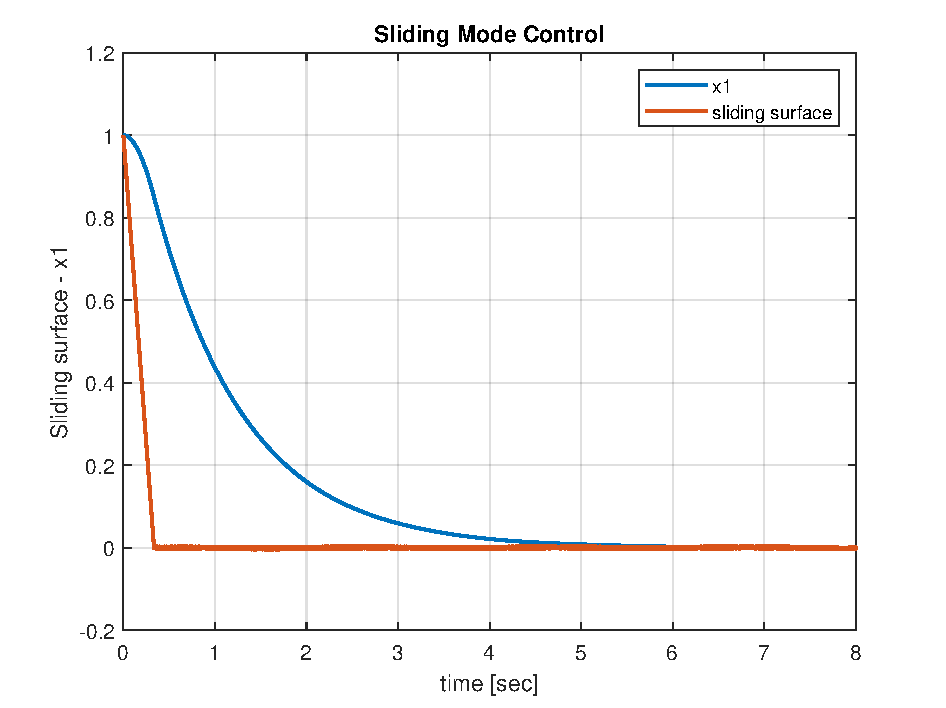
\includegraphics[height=4cm]{./pictures/SMCutkinRoadmap.pdf}
\end{columns}
 \end{frame}
%%% Local Variables:
%%% mode: latex
%%% TeX-master: "SMC4Students"
%%% End:


% *****************************************************************

% <<FF>> ***********************************************************************
% https://www.overleaf.com/learn/latex/Beamer_Presentations:_A_Tutorial_for_Beginners_(Part_2)%E2%80%94Lists,_Columns,_Pictures,_Descriptions_and_Tables#The_Description_Environment
\begin{frame}
  \frametitle{TikZ Test}

  Hello world


% <<FF>> ********************************************************************
% FIGURE: Linear Approximation of the measured curves
% ***************************************************************************
% \begin{figure}[htbp]
  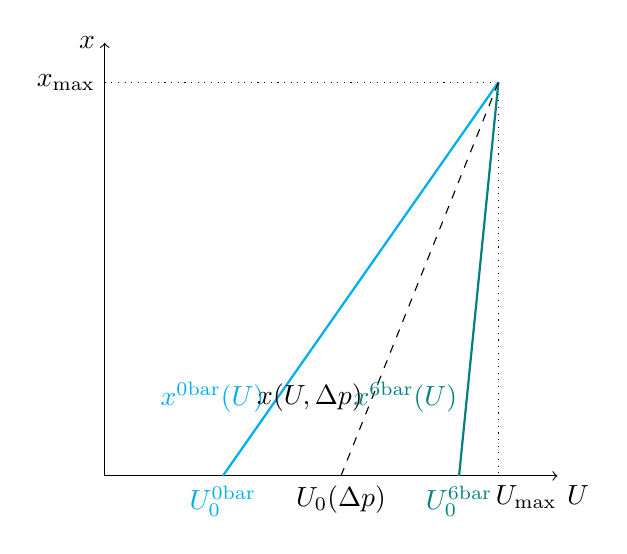
\begin{tikzpicture}[scale=.5]
    % Define the nodes
    \draw [<->] (11.5,0) node[below right] {$U$} -- (0,0) -- (0,11) node[left] {$x$} ; % Coordinates
     %Draw the lines
    \draw [dotted] (0,10) node[left] {$x_{\max}$} -- (10,10) -- (10,0) node [below] {$\qquad U_{\max}$}; % Rechts oben Hilfslinien
    \draw [thick, cyan]  (3,0) node[below]{$U_0^{0\unit{bar}}$} -- (10,10); % 0Bar Linie
    \draw [thick, teal]  (9,0) node[below]{$U_0^{6\unit{bar}}$} -- (10,10); % 6Bar Linie
    \draw [dashed] (6,0) node[below]{$U_0(\Delta p)$} -- (10,10); % 3bar Linie
    \node [cyan, left] at (4.3,2) {$x^{0\unit{bar}}(U)$};
    \node [left] at (6.8,2) {$x(U,\Delta p)$};
    \node [teal, left] at (9.2,2) {$x^{6\unit{bar}}(U)$};    
   \end{tikzpicture}
%   \caption{Illustration of the linear approximation of the measured curves}
%   \label{fig:linapprox}
% \end{figure}

  
 \end{frame}


 
%%% Local Variables:
%%% mode: latex
%%% TeX-master: "SMC4Students"
%%% End:


% <<FF>> ***************************************************
\begin{frame}
\frametitle{References}
% This prints the bibliography on the slide
\printbibliography
\end{frame}


\end{document}